\chapter{Introduction}

\section{Models}

Ledgers have been a central element of commerce since ancient times, and are be used to record a variety of informations, from assets to property, but most importantly how these change hands, that is \textit{transactions}. 

The medium on which transactions have been stored may have changed from clay tablets to hardware storage, but in all this time there haven't been notable innovations to the underlying architecture of the system.
Each financial entity (i.e. banks, governments, financial institutions) manages its own ledgers, with its own technologies and implementative properties, based on their vision, necessities and customers (or, \textit{counterparts}), and in turn, the counterparts keep recorded their own views of the transactions.

This duplication of information between each party partecipating in the transaction drives a need for costly matching between each copy of the information, reconciliation and error fixing. The plurality of technology platforms upon which financial entities rely adds to that, creating more complexity and operational risks, some of which potentially systematic.

Think about the need for a customer to send money to another, from Bank A to Bank B. The difference between infrastructures is such that there's a need for a long process of intercommunication between the two banks before the transaction can end, and that is one of the reasons why there's an inherent slowness to the reception and availability of assets.  \\

Centralized infrastructures were until recently an unavoidable model, as there were few ways to consolidate technologies without effectively consolidating the financial entities themselves. The industry has been moving towards the standardization and sharing of data and some of the business-logic behind the architectures through the delegation of some part of the process to third-parties, but these steps are still lagging behind the evolution of the technology. 

\begin{figure}[t]
    \centering
    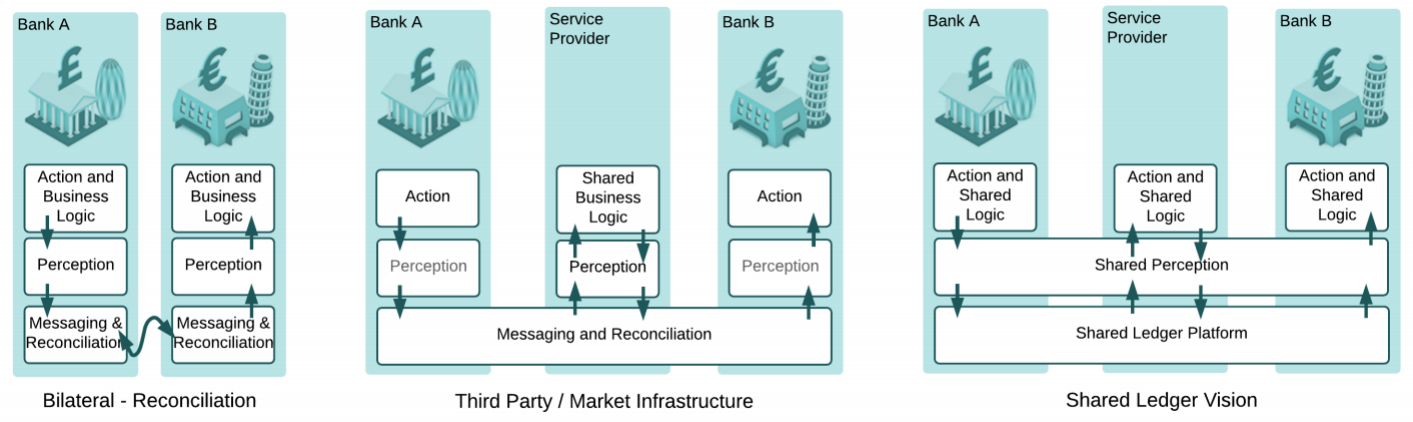
\includegraphics[scale=0.3]{architectures-comparison.png}
    \caption{
        Figure 1: Comparison between architectures from the \cite[cordawhitepaper]. 
        }
\end{figure}
